\documentclass[10pt]{beamer}

\usetheme{CambridgeUS}
\usepackage[english, russian]{babel}
\usepackage[utf8]{inputenc}
\usepackage{caption}
\usepackage{etoolbox}
\usepackage{multicol}
\usepackage{listings}
\usepackage{wasysym}
\usepackage{mathtools}
\DeclarePairedDelimiter\ceil{\lceil}{\rceil}
\DeclarePairedDelimiter\floor{\lfloor}{\rfloor}

\definecolor{mygreen}{rgb}{0,0.6,0}
\lstset{
  basicstyle=\ttfamily\footnotesize,        % the size of the fonts that are used for the code
  breaklines=true,                 % automatic line breaking only at whitespace
  captionpos=b,                    % sets the caption-position to bottom
  commentstyle=\color{mygreen},    % comment style
  keywordstyle=\color{blue},       % keyword style
  stringstyle=\color{red},     % string literal style
  showstringspaces=false,
  morekeywords={include, printf},
  texcl=true     %<---- added
}


\title[\href{https://goo.gl/NRgp8K}{https://goo.gl/NRgp8K} (Term 1)]{Транспортная сеть и максимальный поток}
\author[Гусев Илья, Булгаков Илья]{Гусев Илья, Булгаков Илья}
\institute[МФТИ] 
{Московский физико-технический институт\\*}
\date{Москва, 2019}
\subject{Computer Science}

\begin{document}

\begin{frame}
  \titlepage
\end{frame}

\begin{frame}{Содержание}
\tableofcontents
\end{frame}

\section{Транспортная сеть и поток}

\begin{frame}[fragile]{Транспортная сеть}

Определение. Транспортная сеть — ориентированный граф G=(V,E), в котором
\begin{itemize}
    \item Каждое ребро $(u,v) \in E$ имеет неотрицательную пропускную способность $c(u,v)\geq 0$. 
    \item Выделяются две вершины: источник $s$ и сток $t$ такие, что любая другая вершина сети лежит на пути из $s$ в $t$.
\end{itemize}
Зачем это нужно? Транспортная сеть может быть использована для моделирования, например, дорожного трафика.

\begin{center}
    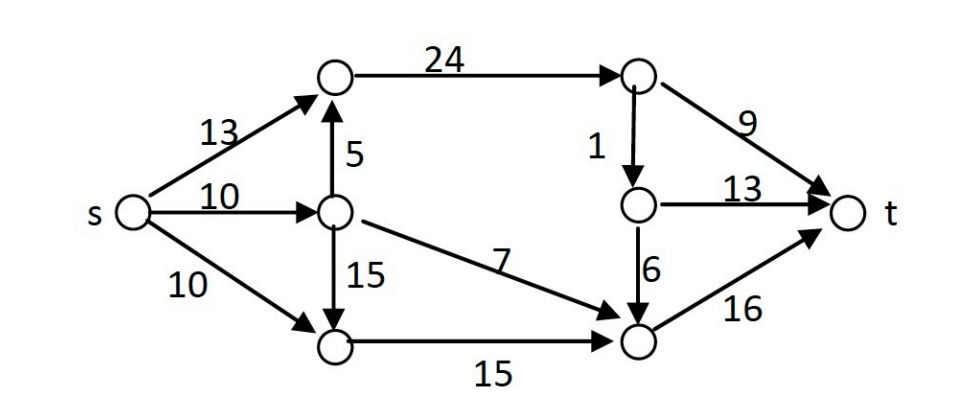
\includegraphics[width=7cm]{Term_2/Source/images/8-transport-network.jpg}
\end{center}

\end{frame}

\begin{frame}[fragile]{Поток в транспортной сети}

Определение. Потоком $f$ в сети $G=(V,E,c)$ называется функция $f:E \rightarrow R$, удоволетворяющая условиям:
\begin{itemize}
    \item $0 \leq f(e) \leq c(e)$ для всех $e \in E$;
    \item $f(v')=f(v*)$ для всех $v \in V$, $v \neq s$, $v \neq t$, где $f(v')= 
    \sum_{w \in v'} f(w,v)$, $f(v*)= \sum_{u \in v*}f(v,u)$.
\end{itemize}

\begin{center}
    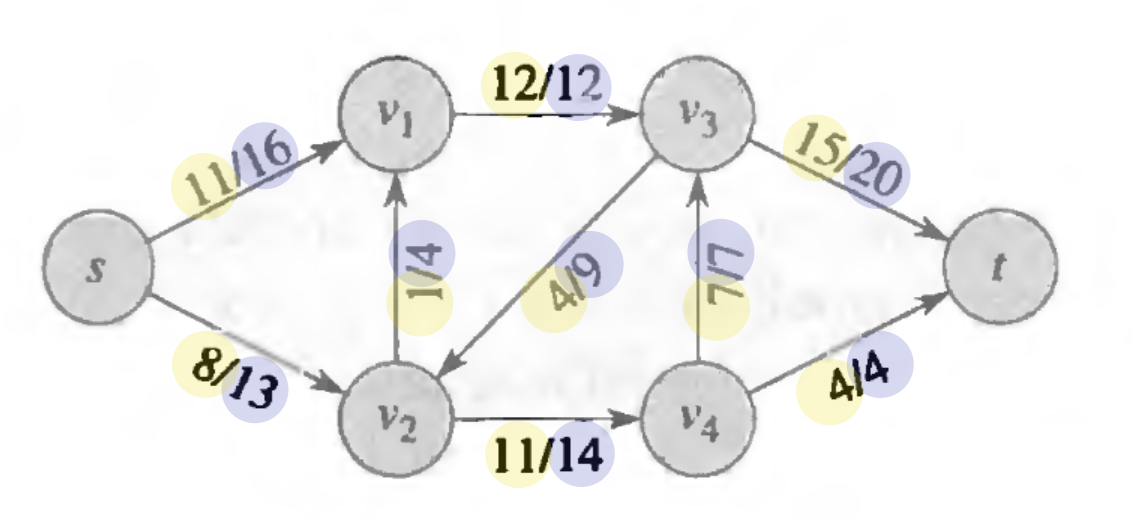
\includegraphics[width=7cm]{Term_2/Source/images/8-flow-colors.png}
\end{center}

\end{frame}

\section{Задача о максимальном потоке}

\begin{frame}[fragile]{Задача о максимальном потоке}

Задача о максимальном потоке заключается в нахождении такого потока по транспортной сети, что сумма потоков из истока, или, что то же самое, сумма потоков в сток максимальна.

\begin{center}
    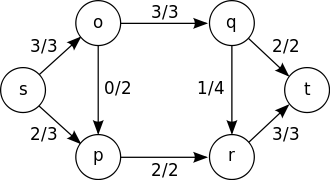
\includegraphics[width=8cm]{Term_2/Source/images/8-flow-rich-networkr.png}
\end{center}


\end{frame}

\begin{frame}[fragile]{Задача о максимальном потоке}

Построение максимального потока
\begin{itemize}
    \item Метод и алгоритм Форда-Фалкерсона
    \item Алгоритм Эдмондса-Карпа
    \item Алгоритм Диница
\end{itemize}

\end{frame}

\section{Метод и алгоритм Форда-Фалкерсона}

\begin{frame}[fragile]{Метод Форда-Фалкерсона}

Описание метода Форда Фалкерсона
\begin{enumerate}
    \item Задаём начальное значение потока $f=0$
    \item while (существует увеличивающий путь $p$)
        \begin{itemize}
            \item Увеличиваем поток $f$ вдоль пути $p$
        \end{itemize}
    \item Возвращаем $f$
\end{enumerate}

\end{frame}

\begin{frame}[fragile]{Метод Форда-Фалкерсона}

Сеть 
\begin{center}
    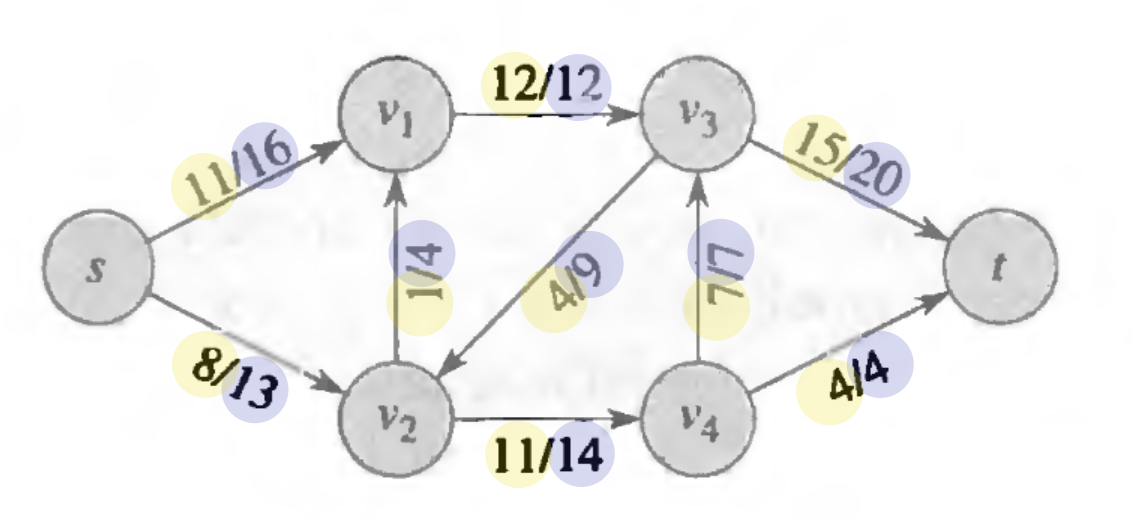
\includegraphics[width=7cm]{Term_2/Source/images/8-flow-colors.png}
\end{center}

Остаточная сеть

\begin{center}
    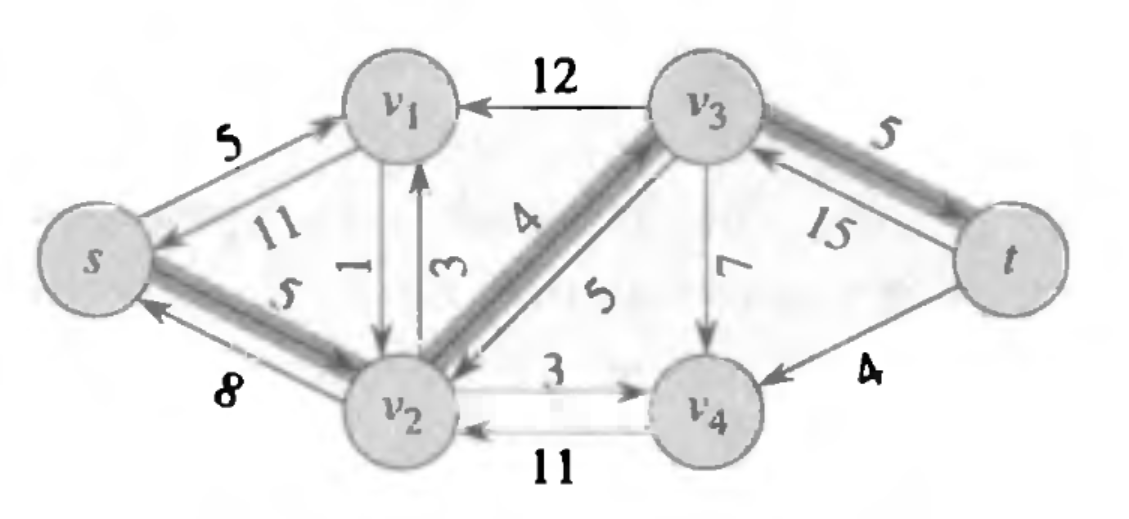
\includegraphics[width=7cm]{Term_2/Source/images/8-flow-residual-network.png}
\end{center}

\end{frame}

\begin{frame}[fragile]{Метод Форда-Фалкерсона}

Увеличивающий путь

\begin{center}
    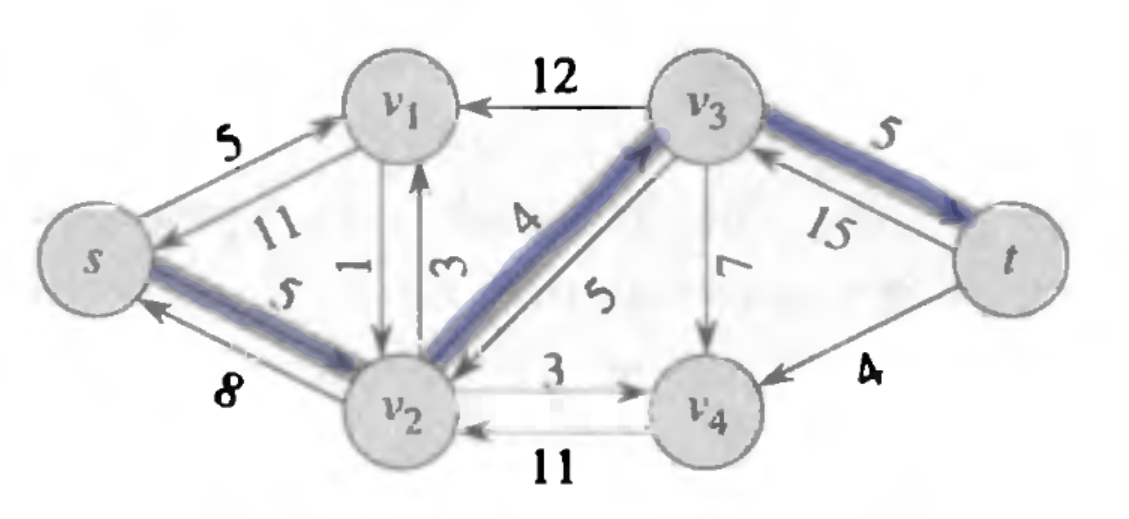
\includegraphics[width=9cm]{Term_2/Source/images/8-flow-augmenting-path.png}
\end{center}

\end{frame}

\begin{frame}[fragile]{Метод Форда-Фалкерсона}

Остаточная сеть и невозможность построить увеличивающий путь

\begin{center}
    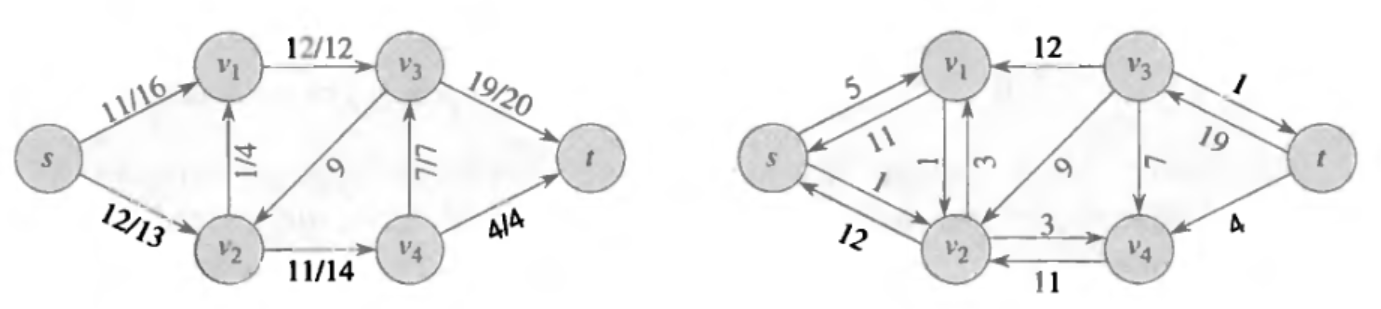
\includegraphics[width=12cm]{Term_2/Source/images/8-flow-residual-network-no-way.png}
\end{center}

\end{frame}

\begin{frame}[fragile]{Метод Форда-Фалкерсона}

Описание базового алгоритма Форда Фалкерсона
\begin{enumerate}
    \item Для каждого ребра $(u,v) \in G$ задаём начальное значение потока $f=0$
    \item \textbf{while} (существует путь $p$ в остаточной сети $G_f$)
        
        \begin{itemize}
            \item Вычисляем $c_f(p) = min\{ c_f(u,v): (u,v)$ содержится в $p$ \}
            \item Для каждого ребра $(u,v)$ в $p$ 
                \begin{itemize}
                    \item \textbf{if} $(u,v) \in E$  $p$ $(u,v).f -= c_f(p) $ 
                    \item \textbf{else} $(u,v).f += c_f(p) $ 
                \end{itemize}
        \end{itemize}
    \item Возвращаем $f$
\end{enumerate}

\end{frame}

\begin{frame}[fragile]{Метод Форда-Фалкерсона}

Сложность алгоритма -- $O( E |f*|)$

Проблемы алгоритма при большой величине потока. Требуется 2млн итераций для нахождения максимального потока.
\begin{center}
    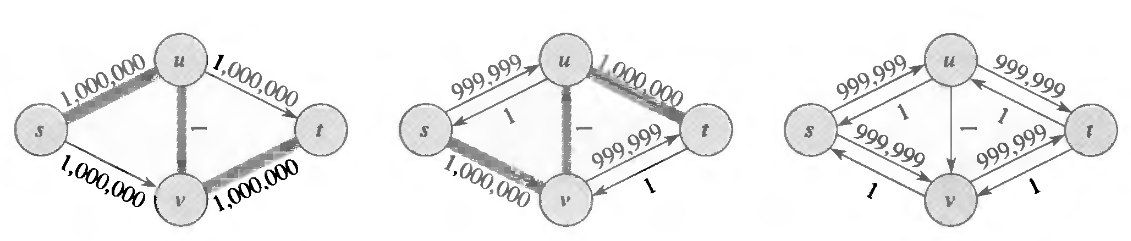
\includegraphics[width=12cm]{Term_2/Source/images/8-ford-falkerson-bad.png}
\end{center}

\end{frame}

\section{Алгоритм Эдмондса-Карпа}

\begin{frame}[fragile]{Алгоритм Эдмондса-Карпа}

Модификация алгоритма Форда-Фалкерсона, в котором вычисление увеличивающего пути $p$ производится как поиск в ширину и выбирается кратчайший путь из $s$ в $t$. Вес ребра принимается за 1.

Сложность алгоритма -- $O( V * E^2)$

\end{frame}

\section{Алгоритм Диница}

\begin{frame}[fragile]{Алгоритм Диница}

\textbf{Блокирующим потоком} в данной сети называется такой поток, что любой путь из истока $s$ в сток $t$ содержит насыщенное этим потоком ребро. Иными словами, в данной сети не найдётся такого пути из истока в сток, вдоль которого можно беспрепятственно увеличить поток.

Блокирующий поток не обязательно максимален. Поток будет максимальным тогда и только тогда, когда в остаточной сети не найдётся $s-t$ пути; в блокирующем же потоке ничего не утверждается о существовании пути по рёбрам, появляющимся в остаточной сети.

\end{frame}

\begin{frame}[fragile]{Алгоритм Диница}

\textbf{Слоистая сеть (layered network)}. 

\begin{center}
    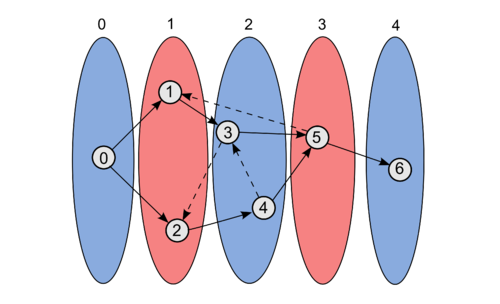
\includegraphics[width=5cm]{Term_2/Source/images/8-layered-network.png}
\end{center}

\begin{itemize}
    \item Определяем длины кратчайших путей из истока s до всех остальных вершин. Назовём уровнем {\rm level}[v] вершины её расстояние от истока. 
    \item Включаем все те рёбра $(u,v)$ исходной сети, которые ведут с одного уровня на какой-либо другой, более поздний, уровень, т.е. {\rm level}[u] + 1 = {\rm level}[v]
    \item Удаляем все рёбра, расположенные целиком внутри уровней, а также рёбра, ведущие назад, к предыдущим уровням.
\end{itemize}

\end{frame}

\begin{frame}[fragile]{Алгоритм Диница}

\textbf{Слоистая сеть (layered network)}. 

\begin{center}
    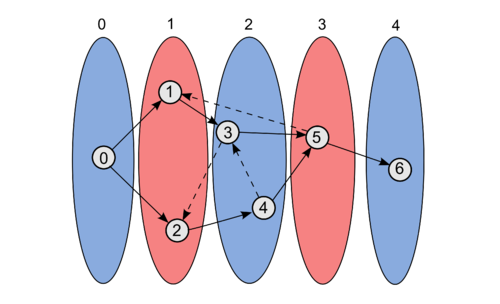
\includegraphics[width=5cm]{Term_2/Source/images/8-layered-network.png}
\end{center}

Слоистая сеть ациклична. Кроме того, любой $s-t$ путь в слоистой сети является кратчайшим путём в исходной сети.

\textbf{Как построить}: для этого надо запустить обход в ширину по рёбрам этой сети, посчитав тем самым для каждой вершины величину {\rm level}[], и затем внести в слоистую сеть все подходящие рёбра.

\end{frame}

\begin{frame}[fragile]{Алгоритм Диница}

Алгоритм представляет собой несколько фаз. 

Фаза алгоритма 

\begin{itemize}
    \item Строим остаточную сеть
    \item По отношению к ней строим слоистую сеть (обходом в ширину)
    \item Ищем произвольный блокирующий поток
    \item Найденный блокирующий поток прибавляется к текущему поток
\end{itemize}

\end{frame}

\begin{frame}[fragile]{Алгоритм Диница}

Поиск блокирующего потока. Возможные реализации:

\begin{itemize}
    \item Ищем пути по одному, пока такие пути находятся. Путь можно найти за O(m) обходом в глубину, а всего таких путей будет O(m) (каждый путь насыщает минимум одно ребро). Получаем $O(E^2)$.
    \item Аналогично предыдущей идее, однако удалять в процессе обхода в глубину из графа все "лишние" рёбра, т.е. рёбра, вдоль которых не получится дойти до стока. Поддерживать в списке смежности каждой вершины указатель на первое неудалённое ребро, и увеличивать этот указать в цикле внутри обхода в глубину. Худший случай $O(V*E)$
\end{itemize}

\end{frame}

\begin{frame}[fragile]{Алгоритм Диница}

Отличие от алгоритма Эдмондса-Карпа: на каждой итерации поток увеличивается не вдоль одного кратчайшего $s-t$ пути, а вдоль целого набора таких путей (ведь именно такими путями и являются пути в блокирующем потоке слоистой сети).

Сложность алгоритма в худшем случае -- $O(E*V^2)$

\end{frame}

\begin{frame}[fragile]{Алгоритм Диница}

\textbf{Пример. Фаза 1}. 

\begin{center}
    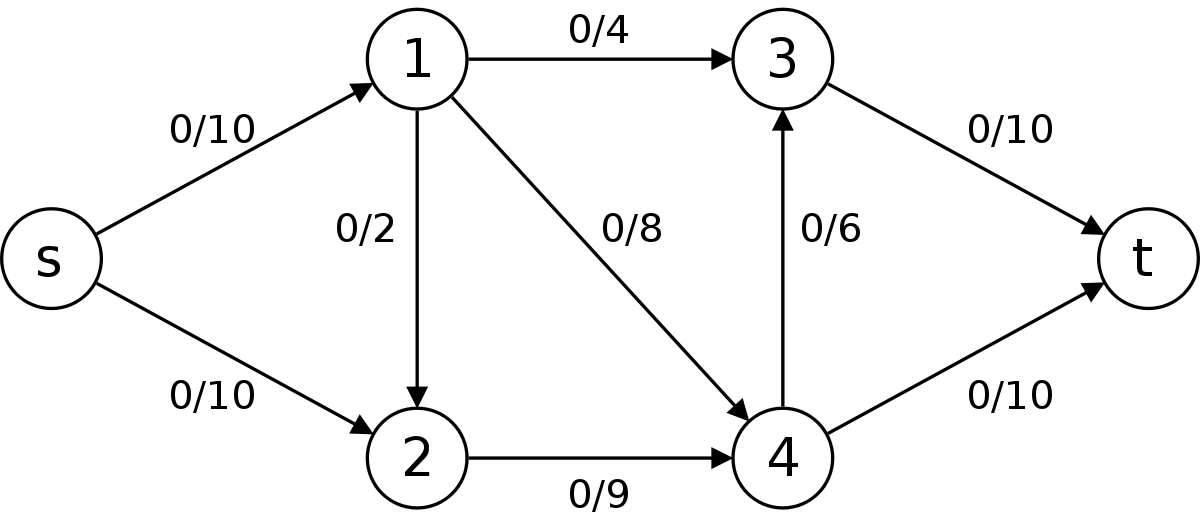
\includegraphics[width=5cm]{Term_2/Source/images/8-dinica-1.png}
\end{center}
\begin{center}
    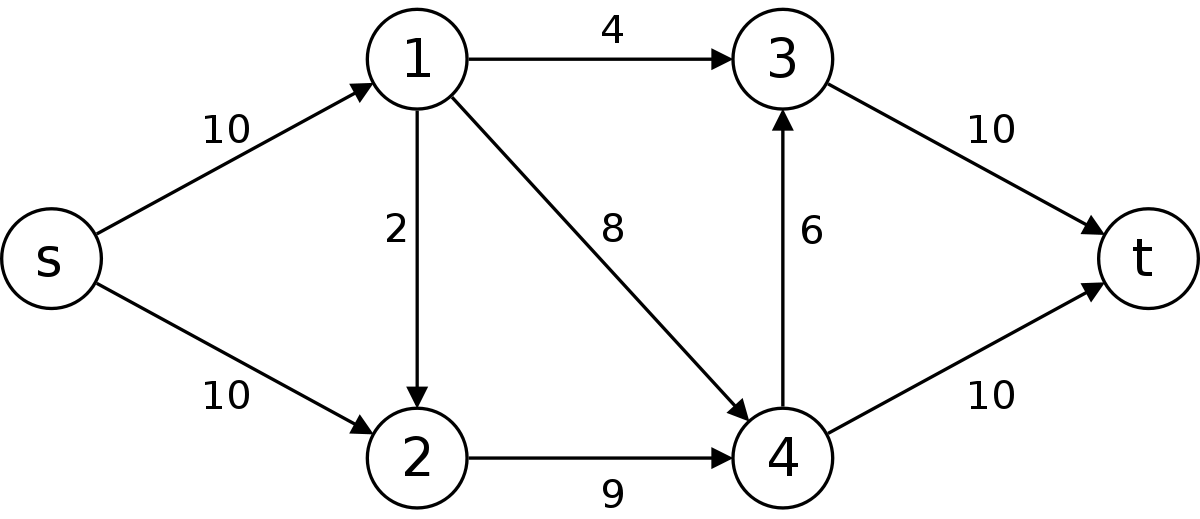
\includegraphics[width=5cm]{Term_2/Source/images/8-dinica-2.png}
\end{center}
\begin{center}
    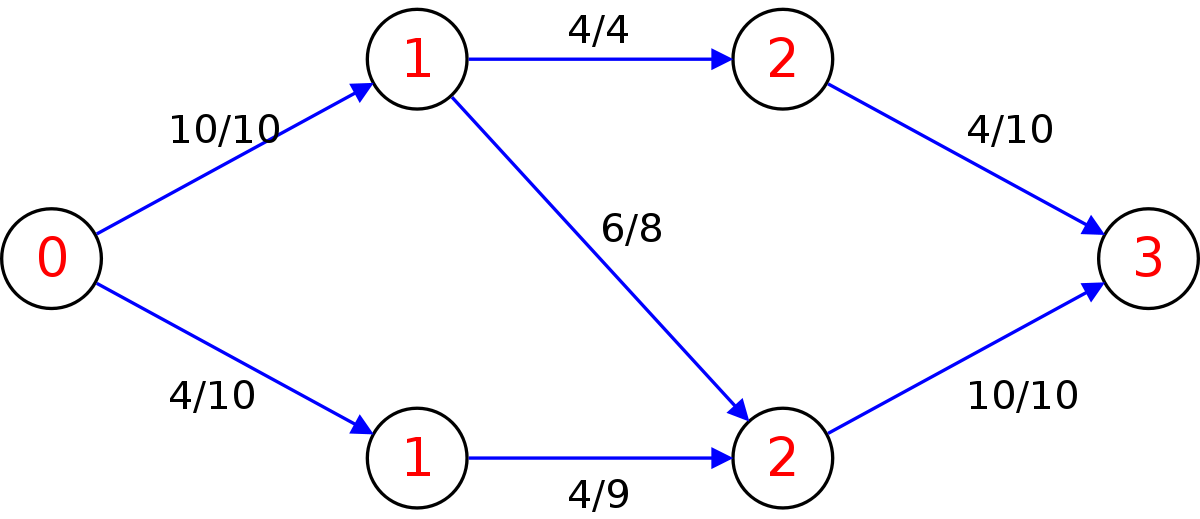
\includegraphics[width=5cm]{Term_2/Source/images/8-dinica-3.png}
\end{center}
\end{frame}

\begin{frame}[fragile]{Алгоритм Диница}

\textbf{Пример. Фаза 2}. 

\begin{center}
    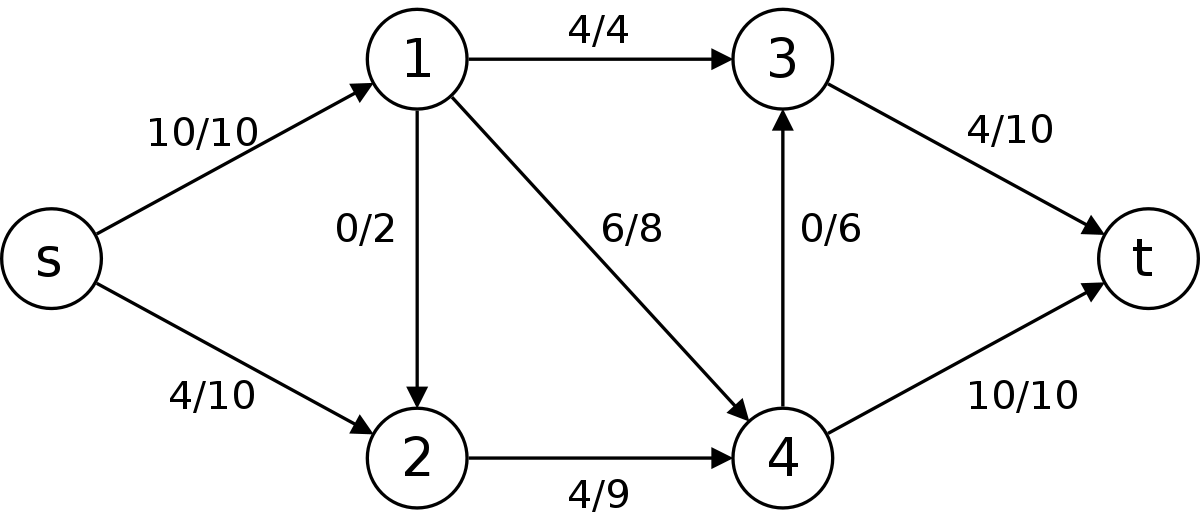
\includegraphics[width=5cm]{Term_2/Source/images/8-dinica-4.png}
\end{center}
\begin{center}
    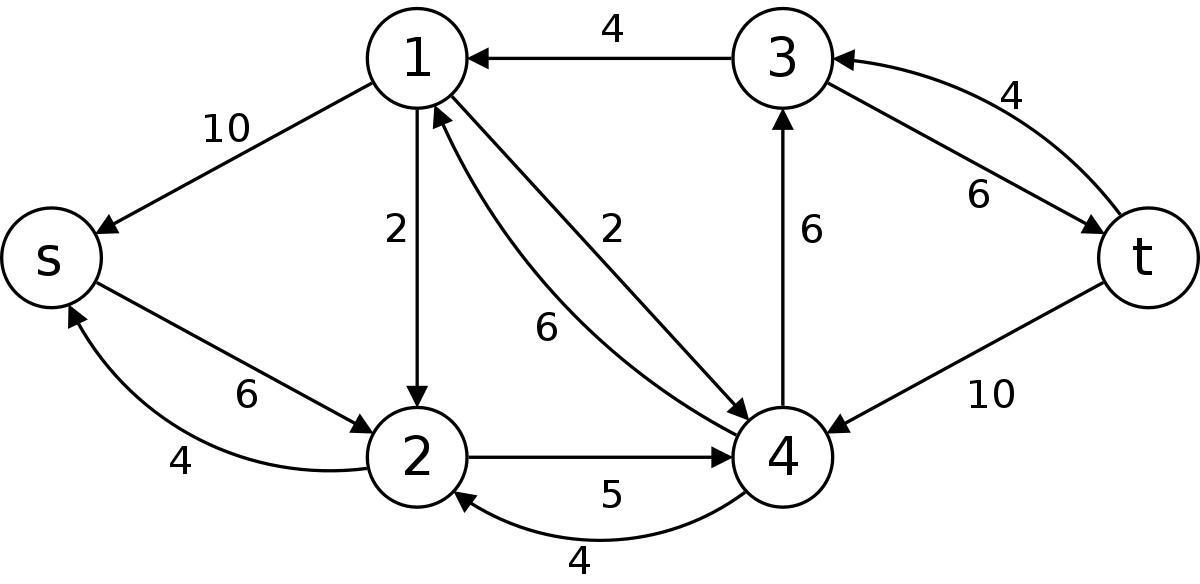
\includegraphics[width=5cm]{Term_2/Source/images/8-dinica-5.png}
\end{center}
\begin{center}
    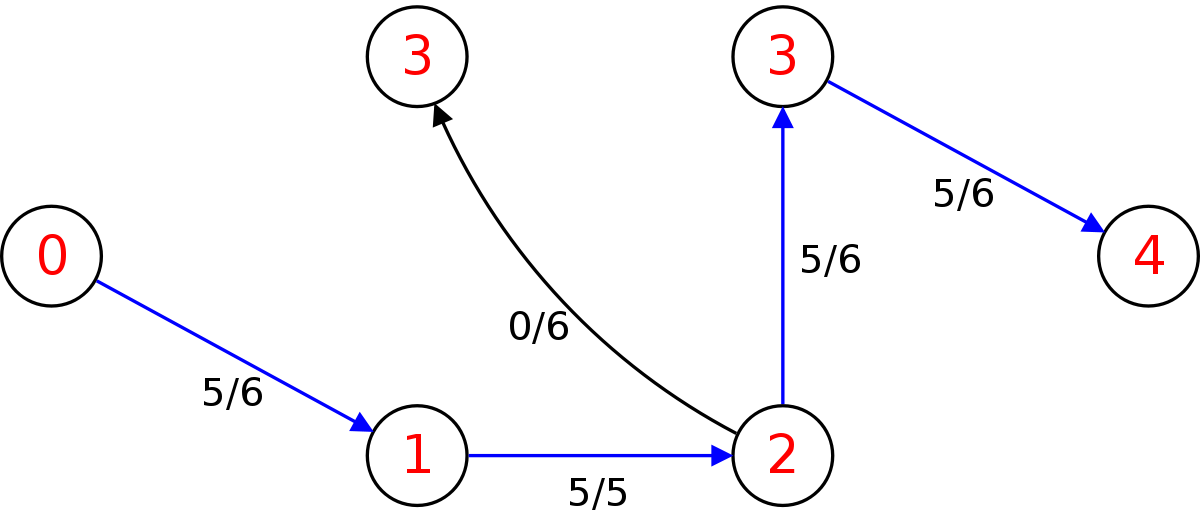
\includegraphics[width=5cm]{Term_2/Source/images/8-dinica-6.png}
\end{center}
\end{frame}


\begin{frame}[fragile]{Алгоритм Диница}

\textbf{Пример. Фаза окончания}. 

\begin{center}
    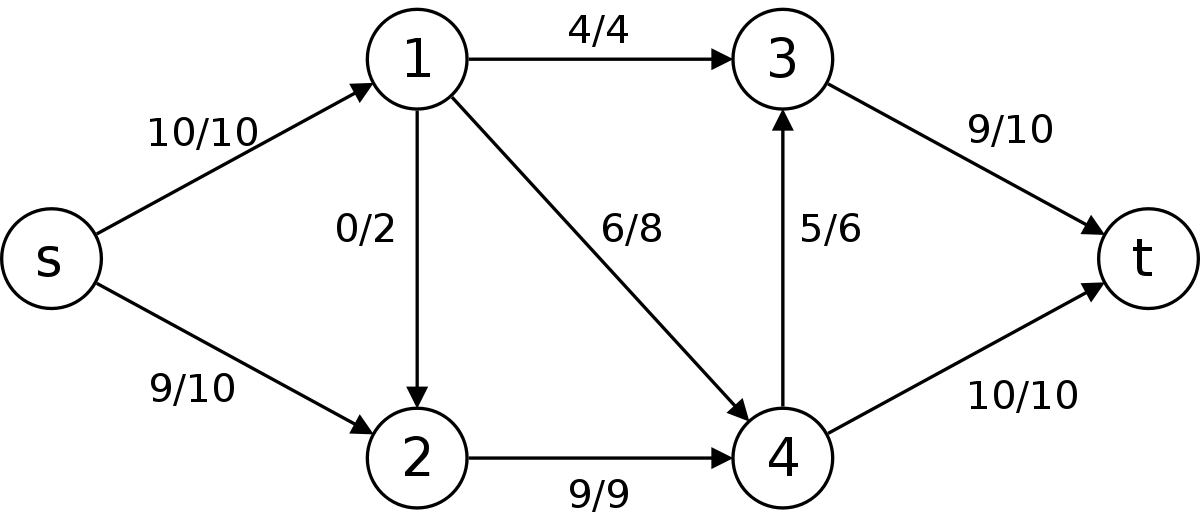
\includegraphics[width=5cm]{Term_2/Source/images/8-dinica-7.png}
\end{center}
\begin{center}
    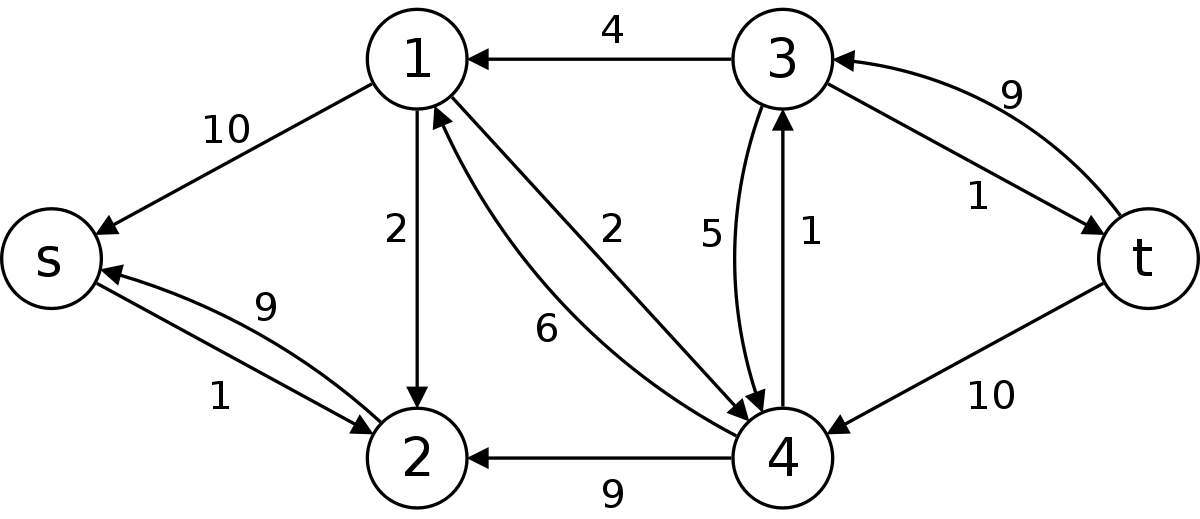
\includegraphics[width=5cm]{Term_2/Source/images/8-dinica-8.png}
\end{center}
\begin{center}
    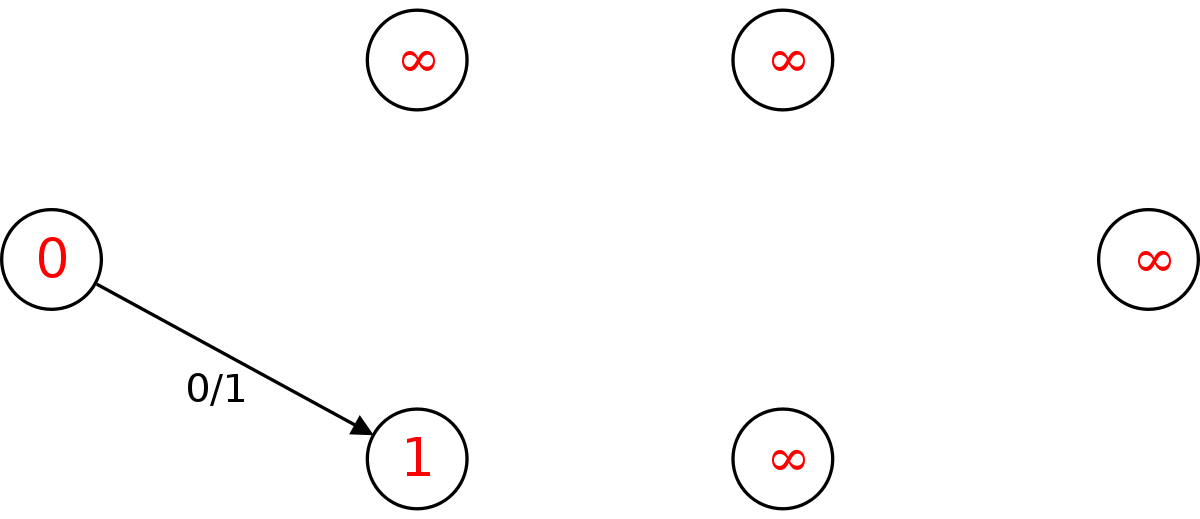
\includegraphics[width=5cm]{Term_2/Source/images/8-dinica-9.png}
\end{center}
\end{frame}

\appendix

\begin{frame}[allowframebreaks]
  \frametitle<presentation>{Полезные ссылки}
    
  \begin{thebibliography}{10}
{
  \beamertemplatebookbibitems
  % Start with overview books.

  \bibitem{neerc}
  \texttt{E-maxx: описание алгоритма Диница}
  \newblock \href{http://e-maxx.ru/algo/dinic }{\texttt{http://e-maxx.ru/algo/dinic}}
  
  \bibitem{neerc}
  \texttt{Методы применения алгоритма нахождения максимального потока в сети}
  \newblock \href{https://habr.com/ru/post/102367/ }{\texttt{https://habr.com/ru/post/102367/}}
  
}
  \end{thebibliography}
  \end{frame}

\end{document}


